\documentclass[11pt, onecolumn]{article}
\usepackage{hyperref}
\usepackage{url}
%\usepackage{mathpazo,mathrsfs}
%\usepackage[T1]{fontenc}

%\usepackage[usenames,dvipsnames]{color}
\usepackage{stmaryrd} \usepackage{url} \usepackage[latin1]{inputenc}
\usepackage{graphicx}% Include figure files
\usepackage{amssymb} \usepackage{subfigure} \usepackage{amsmath}
\usepackage{amsthm}
\usepackage{dcolumn}% Align table columns on decimal point
\usepackage{bm}% bold math
\usepackage{color}
\usepackage{mathtools}


%\usepackage{algorithm} \usepackage{algorithmic}
\usepackage[noline,boxed]{algorithm2e}

\newcommand{\alert}[1]{\textcolor{red}{#1}} \newcommand{\vect}[1]{\boldsymbol{#1}}
\newcommand{\todo}[1]{\vspace{5 mm}\par \noindent \framebox{\begin{minipage}[c]{8cm} \tt
      #1
    \end{minipage}}\vspace{5 mm}\par}

\newcommand{\STATE}{\quad}
\newcommand{\COMMENT}[1]{{\sl (#1)}}
\newcommand{\RETURN}{\tb{Return }}

\newtheorem{theorem}{Theorem}[section]
\newtheorem{statement}[theorem]{Statement}
\newtheorem{proposition}[theorem]{Proposition}
\newtheorem{lemma}[theorem]{Lemma}
\newtheorem{corollary}[theorem]{Corollary}
\newtheorem{question}[theorem]{Question}
\newtheorem{remark}[theorem]{Remark}
\newtheorem{conjecture}{Conjecture}
\newtheorem{claim}[theorem]{Claim}
\newtheorem{condition}[theorem]{Condition}
\newtheorem*{subproblem*}{Subproblem}
\newtheorem{definition}[theorem]{Definition} \newtheorem{example}{Example}
\newtheorem{assumption}{Assumption} \newtheorem{scenario}{Scenario}
\newtheorem{step}{Step} \newtheorem{steps}{Step} \newtheorem{stp}{Step}
\newtheorem{stps}{Step} \newtheorem{problem}{Problem}

%\newenvironment{proof}[1][Proof]{\begin{trivlist}
%\item[\hskip \labelsep {\bfseries #1}]}{\end{trivlist}}


\usepackage{hyperref}

%\renewcommand{\algorithmicrequire}{\textbf{Input:}}
%\renewcommand{\algorithmicensure}{\textbf{Output:}}
%\renewcommand{\algorithmireturn}{\textbf{Return:}}



%\usepackage[dvips]{graphicx}
% \usepackage{amsfonts,mathrsfs,amsfonts, array, geometry}
% \usepackage{graphicx,amsmath,amssymb,multirow} \setcounter{MaxMatrixCols}{30}%
% \usepackage[usenames]{color} \usepackage[usenames, dvipsnames]{xcolor}
% \usepackage{epstopdf}\usepackage{framed}
% \usepackage{algpseudocode}
% \usepackage{ulem}

% \newtheorem{Thm}{Theorem} \newtheorem{Lem}{Lemma} \newtheorem{Cor}{Corollary}
% \newtheorem{Def}{Definition} \newtheorem{Exam}{Example} \newtheorem{Alg}{Algorithm}
% \newtheorem{Prob}{Problem} \newtheorem{Rem}{Remark} \newtheorem{Proof}{Proof}
% \newtheorem{Prop}{Proposition} \newtheorem{Assump}{Assumption}

\newcommand{\mc}{\mathcal}
\newcommand{\mb}{\mathbf} \newcommand{\mbb}{\mathbb} \newcommand{\wt}{\widetilde}
\newcommand{\fa}{\forall} \newcommand{\tc}{\textcolor} \newcommand{\tb}{\textbf}
\newcommand{\tx}{\text} \newcommand{\tcws}{\textcolor{WildStrawberry}}
\newcommand{\tcbl}{\textclor{blue}}
\newcommand{\p}{\partial}
\newcommand{\dr}{\text{d}}
\newcommand{\bs}{\boldsymbol}
\newcommand{\ot}{\otimes}

\newcommand{\ta}{\theta}
\newcommand{\Ta}{\Theta}

\newcommand{\Proj}{\mbox{Proj}}
\newcommand{\R}{\mbb R}
\newcommand{\C}{\mbb C}
\newcommand{\Z}{\mbb Z}
\newcommand{\E}{\mbb E}

\newcommand{\ul}{\underline}
\newcommand{\ol}{\overline}
\newcommand{\wh}{\widehat}
\newcommand{\prj}{\tx{Proj}}
% \newcommand{\mog}{Gaussian mixture model}
\newcommand{\mog}{mixture of Gaussians }
% \newcommand{\mog}{MoG}
\newcommand{\vc}{\tx{vec}}
\newcommand{\mt}{\tx{mat}}
\newcommand{\diag}{\tx{diag}}
\newcommand{\poly}{\tx{poly}}
\newcommand{\cond}{\tx{cond}}
\newcommand{\ep}{\tx{exp}}
\newcommand{\lt}{\left}
\newcommand{\rt}{\right}

\newcommand{\defeq}{\vcentcolon=}
\newcommand{\eqdef}{=\vcentcolon}
\newcommand{\od}{\odot}

%\linespread{1}
%\let\labelindent\relax
\usepackage{enumitem}
\usepackage[margin=1in]{geometry}

\newcommand{\qq}[1]{{\color{magenta}{(#1)}}}
\newcommand{\rd}[1]{{\color{red}{ #1}}}
\newcommand{\bl}[1]{{\color{blue}{ #1}}}
\iffalse
\fi

\begin{document}
\title{controller validation for uncertain systems}
\date{\today}

%\maketitle
%\thispagestyle{empty}
%\pagestyle{empty}

% \begin{abstract}
% \end{abstract}
% \begin{keywords}
% \end{keywords}

\setcounter{page}{1}

\section{Example of tracking}

\paragraph{Step 1}
Open loop id for unknown plant $P$. Run experiment to obtain (input, output) sequence
$(s,v)$.
\begin{figure}[h!]
  \centering
  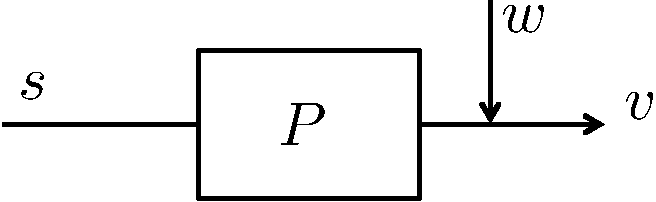
\includegraphics[width=.3\linewidth]{sys3.pdf}
\end{figure}

Assume the measurement noise $w$ in a bounded set with IQC description $\mc Q_w$. Convert the
observation to IQCs about the plant. For example, if we parameterize the plant by its impulse
response $p$, the observation gives the constraint:
\begin{align*}
  ( v - p*s)\in \mc Q_w.
\end{align*}

\paragraph{Step 2}
Place the candidate controller $K$ in the closed loop. Run experiment to obtain (reference, output)
sequence $(r, y)$.
\begin{figure}[h!]
  \centering
  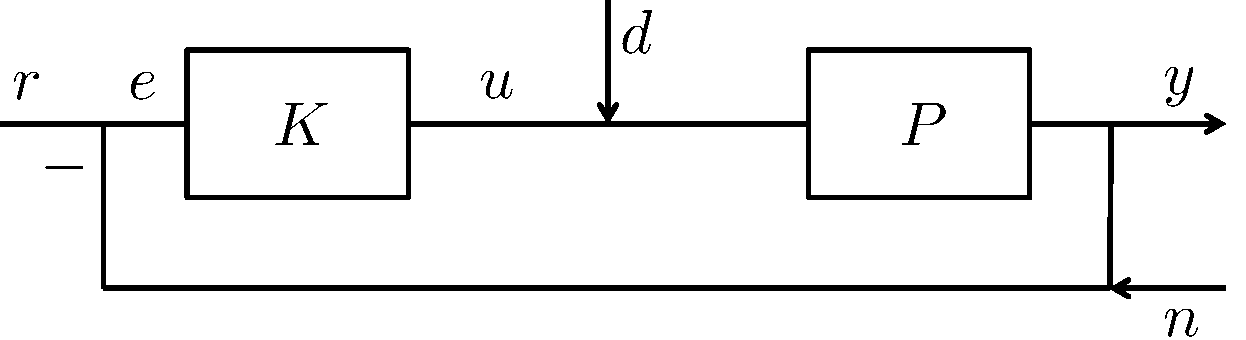
\includegraphics[width=.5\linewidth]{sys2.pdf}
\end{figure}


Given the constraint of the uncertain plant from Step 1, the disturbance $d$ and the measurement
noise $n$ as $\mc Q_d$, $\mc Q_n$. Let $Q_{T,\gamma}$ denote the achieved performance of $(r,y)$
with parameter $\gamma$.

The feasibility problem for validation of $K$ is as follows: Does there exist noise signal $(d, n)$
and impulse response of the plant $p$ such that:
\begin{align*}
  & (r,y)\in\mc Q_{T,\gamma}, \quad\tx{(tracking performance achieved)}
  \\
  & e = r-(y+n), \quad u = K e, \quad y = p * (u+d),  \quad\tx{(signals)}
  \\
  & d\in\mc Q_d, \quad n\in\mc Q_n,  \quad (v-p*s )\in\mc Q_w. \quad\tx{(constraints satisfied)}
\end{align*}

Similarly, the synthesis problem of $K$ is as follows:
\begin{align*}
  &\min_{K\in\mc K} \gamma
  \\
  s.t.& \tx{ the above hold}
\end{align*}


\paragraph{Algo}
When the constraints are IQCs, turn it into LMI.

\paragraph{Sample complexity}
This is the worst case type analysis.

Given $M$ observed roll-outs for step 1, we can obtain tighter constraints of $P$, which converges
to the underlying truth, and the optimal solution in the second step also converges to the optimal
controller with respect to the true plant $P$. Establish the asymptotic convergence, and then finite
sample rate.



\paragraph{Naive questions}
Why not replace Step 2 with IQC synthesis? why not replace Step 1 with point estimator plus
uncertainty set? Advantage compared to existing 2-step ID and robust control?

\newpage



\section{Setup}

\subsection{Basic idea}

Given:
\begin{itemize}
\item The part of plant that is known a priori, denoted by $P$.
\item Support of the of the unknown part of the plant $\Delta$: an {\em initial} description in the
  form of integral quadratic constraints on its input-output pair $(v,s)\in \mc Q_\Delta = \{Q_1,\dots, Q_L\}$.
  % (why not ssv or coprime factor)
\item Support of the controller $K$: a (discrete) set of candidate controllers $K \in \mc K = \{K_1,\dots,
  K_M\}$.
\item Support of the unobserved exogenous noise $w$: a bounded set in the form of IQCs $w\in \mc
  Q_{W}$.
\end{itemize}
Goal: learn about the system so that we can find a controller $K\in\mc K$ which stabilizes the
system and optimizes the $\ell_2$ gain $\|T_{w\to y}\|_{\infty}$.

\paragraph{}
The basic idea of ``controller invalidation'' is as follows.


\begin{enumerate}
\item

Consider closed-loop system with a candidate controller $K\in\mc K$ in place.

Given $P, \mc Q_{\Delta}, \mc Q_{W}$, given length $T$ observation $(u_t, y_t, z_t)_{t=1}^{T}$
generated by the closed loop system, solve the following feasibility problem.

Does there exist signal $(w_t, v_t, s_t)_{t=1}^{T}$ such that the following holds:
\begin{enumerate}
\item {(in time domain)}
  \begin{align*} (z,y,v) = P (u,w,s), \quad u = K z.
  \end{align*}
  Let $F_u(P,K)$ denote the linear fractional transformation, the two time domain equalities are
  equivalent to
  \begin{align*} (y,v) = F_u(P,K) (w,s).
  \end{align*}

\item IQCs for system  uncertainties are satisfied:
  \begin{align*} & w\in\mc Q_W, \quad (v,s) \in \mc Q_{\Delta}
  \end{align*}

\item Performance achieved, namely $\|T_{w\to y}\|_{\infty} \le \gamma$. Note that this closed loop
  constraint can also be described as a IQC $\mc Q_{cl}$ for the pair of signal $(w,y)$:
  \begin{align*}
    (w,y) \in \mc Q_{cl}.
  \end{align*}

\end{enumerate}
These can be turned into an LMI.

% try to invalidate $K$.

\item If we cannot find such $(w,v,s)$, we should rule out $K$ from $\mc K$, because there does not
  exist $\Delta$ and $w$ in the uncertainty set such that $K$ is feasible.

\item In the event that we find such $(w,v,s)$, namely we can find some $w$ and  $\Delta$ in the
  uncertainty set for which $K$ is feasible, we should keep $K$ in $\mc K$.

\item Moreover, for each $K_i\in\mc K$, we can potentially identify a set of $\Delta$ that are
  consistent with the observation for some $w\in\mc Q_{w}$. Denote it by $\Delta_{K_i}$.
  \\
  Find the tightest IQC description for the set $\cap_i \Delta_{K_i}$ and denote it by $\mc
  Q_{\Delta}'$.  Can we confidently rule out the subset of $\Delta$ in $\mc Q_{\Delta} \backslash
  \mc Q_{\Delta}'$?  No system in this subset can generate the observed sequences.

\end{enumerate}

\tb{Remark:}
We need to do this test for every $K$ in the discrete set $\mc K$ to determine whether to keep it or
throw it out. If more than one $K$ is left, we can try:
\begin{itemize}
\item Get new observations for each $K$ with the same setup. Run the same invalidation procedure.
\item With the same observation, search for better performance so that sub-optimal controllers would
  be ruled out.
\item Impose more IQCs (obtained from observation data) to shrink the uncertainty set of $\Delta$.
\end{itemize}



\begin{figure}[h!]
  \centering
  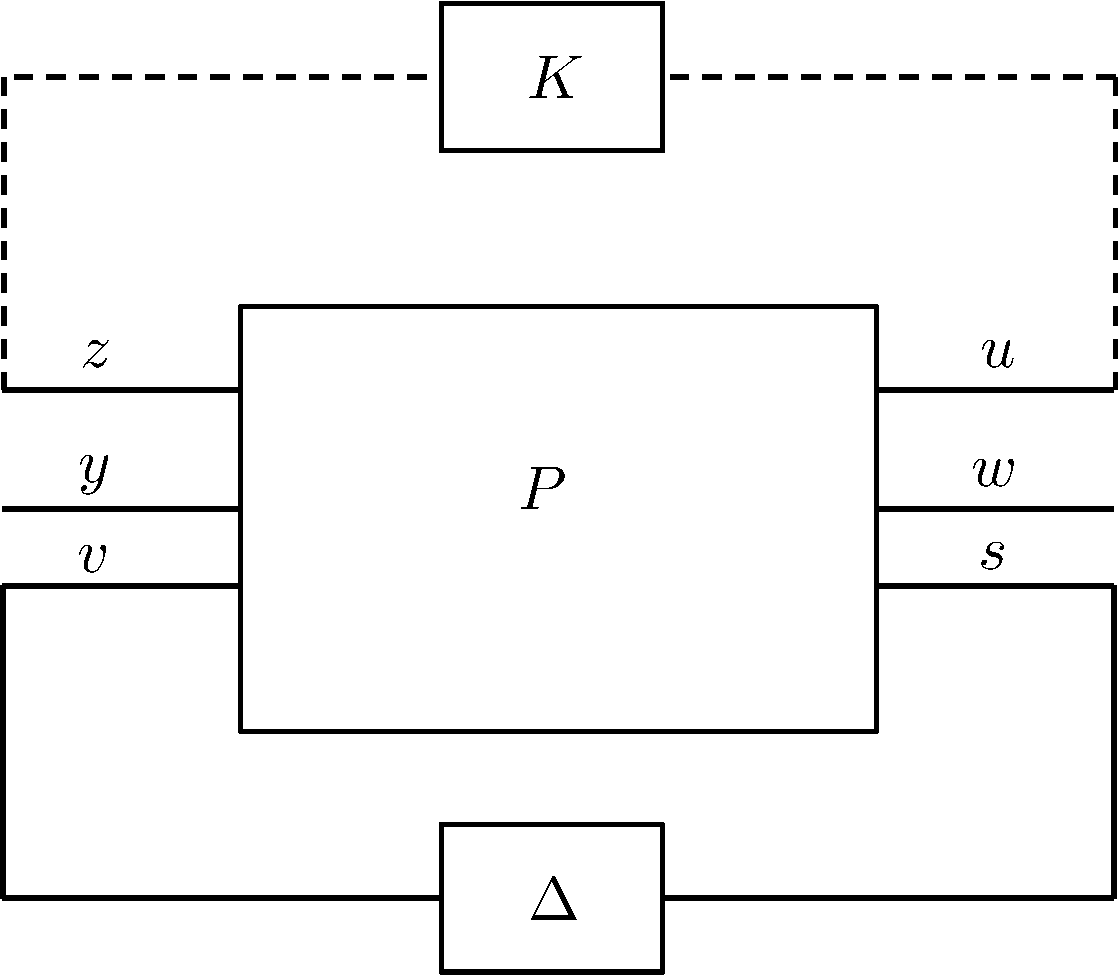
\includegraphics[width=.4\linewidth]{sys1.pdf}
\end{figure}




\section{Discussions}

From the Poolla paper (Time domain approach to model validation), only the unstructured uncertainty
set (convex ball) can be treated. More complicated IQC, and how to obtain more complicated IQC from data?


Naive questions
\begin{enumerate}
\item how does this approach compare to controller synthesis with the IQC for $\Delta$? -- we can
  use the observation sequences without id + control.
\end{enumerate}


After studying the 0-th order question.
\begin{enumerate}
\item Start with a compact set for $\mc K$, we want to test one instance of $K$ and be able to rule
  out a measurable subset of $\mc K$.
\item Incorporate the information in the observation sequences to get a finer description of the
  uncertainty set $\Delta$ in terms of more IQCs in $\mc Q_{\Delta}$, which would give us more
  invalidation power.
\item Experiment design. Note that in the closed loop id, choosing a particular controller $K$
  determines the $u$ input sequence. We want to select a controller $K\in \mc K$ so that we can
  shave of a large portion of $\mc K$ with the invalidation procedure.
\end{enumerate}






\bibliographystyle{plain}
\bibliography{invalid}

\end{document}
